\newpage
\pagenumbering{arabic}
\setcounter{page}{45}


\hline
\begin{center}
    \textbf{ПРАКТИКУМ АБИТУРИЕНТА}
\end{center}
\hline
\begin{LARGE}\begin{flushleft}
    \textbf{ПИСЬМЕННЫЙ ЭКЗАМЕН\\
    ПО МАТЕМАТИКЕ\\
    НА МЕХМАТЕ МГУ В 1970 ГОДУ}
\end{flushleft}\end{LARGE}

\begin{flushright}
\textbf{Н.Н. Колесников}
\end{flushright}

\large
\begin{changemargin}{0.7 cm}{0.5 cm} 
\begin{justify}
\textbf{В «Кванте» № 2 за 1970 год была напечатана статья Н. С. Бахвалова м Н. Н. Кузнецова о письменном экзамене по математике на мехмате МГУ в 1969 году. Хотелось бы, не повторяя сделанные там замечания о характере этого экзамена, подчеркнуть некоторые его особенности
в 1970 году.}
\end{justify}
\end{changemargin}

\normalsize
\setlength{\parindent}{0.5cm}
\begin{justify}
\begin{multicols*}{2}
 {Задачи, предложенные поступавшим, еще раз подтверждают положение о том, что успешное их решение доступно любому абитуриенту, твердо усвоившему школьную программу, а не только выпускникам математических школ. Вы увидите, что эти задачи не содержат «подводных камней» или «ловушек», а требуют четкого понимания основных разделов программы по математике для поступающих в вузы и определенных навыков в технике математических выкладок и решении простейших уравнений, неравенств и геометрических задач.

Естественно, что такая «стандартность» задач предполагает повышение требований к оценке их решений, требований к умению доводить решение до конца, а неограничиваться наметками на решение. Удовлетворительная оценка (три) ставилась в 1970 году за доведенное до конца правильное решение любых двух или трех задач, хорошая (четыре) — любых четырех
задач, отличная (пять) — пяти задач. На решение задания (набора из пяти задач — варианта) отводилось 4 астрономических часа.

Перейдем к разбору одного из вариантов письменного экзамена по математике, коротко останавливаясь на наиболее характерных ошибках, встретившихся в работах поступавших на механико-математический факультет.
\setlength{\parindent}{0cm}

\breakline
\small
\begin{center}
Вариант 1
\end{center}
1. Решить неравенство
\[-\log_\frac{1}{2}(1 + \cos{3x}) \leq 2 + \log_2 (\frac{1}{4} - \cos{x}) \]
2. Найти все действительные решения системы
\begin{equation*}
    \begin{cases}
      y^{2} - |xy| + 2 = 0 ,\\8 - x^{2} = (x + 2y)^{2}.
      \end{cases}
\end{equation*}
3. Три гонщика A, B и C, стартовав одновременно, движутся с постоянными скоростями в одном направлении по кольцевому шоссе. В момент старта гонщик B находится перед гонщиком А на расстоянии $^1/_3$  длины шоссе, а гонщик С - перед гонщиком В на таком же расстоянии. Гонщик А впервые догнал В в тот момент, когда В закончил свой первый круг, а еще через 10 минут А впервые догнал гонщика С. Гонщик В тратит на круг на 2,5 минуты меньше, чем С. Сколько времени тратит на круг гонщик А?

4. На диагонали AC выпуклого четырехугольника ABCD находится центр окружности радиуса r, касающейся сторон AB, AD и BC. На диагонали BD находится центр окружности такого же радиуса r, касающейся сторон BC, CD, AD. Найти площадь четырехугольника ABCD, зная, что указанные окружности касаются друг друга внешним образом.

5. Шар радиуса r касается плоскости Р в точке А. Прямая l образует с плоскостью P
}
\end{multicols*}
\end{justify}

\newpage
\pagestyle {empty}

\begin{table}[]
\begin{adjustwidth}{-1cm}{-1cm}
\centering
\caption*{Таблица 2}
\begin{tabular}{cccll}
\cline{1-4}
\multicolumn{1}{|c|}{\multirow{2}{*}{\begin{tabular}[c]{@{}c@{}} \small Уравнения прямых, на пересечении \\ \small которых лежит вершина\end{tabular}}}                                            & \multicolumn{2}{c|}{\begin{tabular}[c]{@{}c@{}}\small Координаты\\ \small вершины\end{tabular}}                                                                                           & \multicolumn{1}{l|}{\multirow{2}{*}{ \small Значения функции 4х + 3у в вершине}}                                                                                                              &  \\ \cline{2-3}
\multicolumn{1}{|c|}{}                                                                                                                                                              & \multicolumn{1}{c|}{ \small х}                                                               & \multicolumn{1}{c|}{\small y}                                                               & \multicolumn{1}{l|}{}                                                                                                                                                                 &  \\ \cline{1-4}
\multicolumn{1}{|c|}{\begin{tabular}[c]{@{}c@{}} \small x = 0, 2x + y = 10\\ \small 2x + y = 10, x + y = 8\\  \small x +y = 8, 3x + 7y = 42\\  \small 3x + 7y = 42, x + 5y = 20\\ \small x + 5y = 20, y = 0\end{tabular}} & \multicolumn{1}{c|}{\begin{tabular}[c]{@{}c@{}} \small 0\\ \small 2\\ \small 3,5\\ \small 8,75\\ \small 20\end{tabular}} & \multicolumn{1}{c|}{\begin{tabular}[c]{@{}c@{}} \small 10\\ \small 6\\ \small 4,5\\ \small 2,25\\ \small 0\end{tabular}} & \multicolumn{1}{c|}{\begin{tabular}[c]{@{}c@{}} \small 4 \cdot 0 + 3 \cdot 10 = 30\\ \small 4 \cdot 2 + 3 \cdot 6 = 26\\ \small 4 \cdot 3,5 + 3 \cdot 4,5 = 27,5\\ \small 4 \cdot 8,75 + 3 \cdot 2,25 = 41, 75\\ \small 4 \cdot 20 + 3 \cdot 0 = 80\end{tabular}} &  \\ \cline{1-4}
\multicolumn{1}{l}{}                                                                                                                                                                & \multicolumn{1}{l}{}                                                                 & \multicolumn{1}{l}{}                                                                 &                                                                                                                                                                                       & 

\end{tabular}
\end{adjustwidth}
\end{table}


\begin{table}[H]
\caption*{Таблица 3}
\begin{tabular}{|c|c|c|}
\hline
Уравнение прямой &
  \begin{tabular}[c]{@{}c@{}} \small Точки на осях координат, через которые\\ \small проходит прямая\end{tabular} &
  \begin{tabular}[c]{@{}c@{}} \small Тангенс \\ \small  угла нак-\\ \small лона пря-\\ \small мой\end{tabular} \\ \hline
\begin{tabular}[c]{@{}c@{}} \small y = 0\\ \small 2x + 8y = 32\\ \\  \small x + 2y = 12\\ \\ \small 3x + 4y = 36\\ \small 3x + y = 15\\ \small x=0\\ \small 3x + 12y = c\end{tabular} &
  \begin{tabular}[c]{@{}c@{}} \small (0,4), (16,0)\\ \\ \small (0,6), (12,0)\\ \\ \small (0,9), (12,0)\\ \small (0,15), (5,0)\\ \\ \small (0, ^c/_{12}), (^c/_3, 0)\end{tabular} &
  \begin{tabular}[c]{@{}c@{}}0\\ \small ^1/_4\\ \\ \small ^1/_2\\ \\ \small ^3/_4\\ \small 3\\ \small \infty\\ \small ^1/_4\end{tabular} \\ \hline
\end{tabular}
\end{table}
\newpara

\begin{justify}
\begin{multicols}{2}
\colchunk{
Множество допустимых точек изображено на рисунке 11, из которого видно, что прямая х + 2у = 12 лежит целиком вне этого множества. Таким образом, сторонами этого множества служат лучи осей координат и отрезки  трех оставшихся прямых. 

\multicolfloat{}{}{
\centering
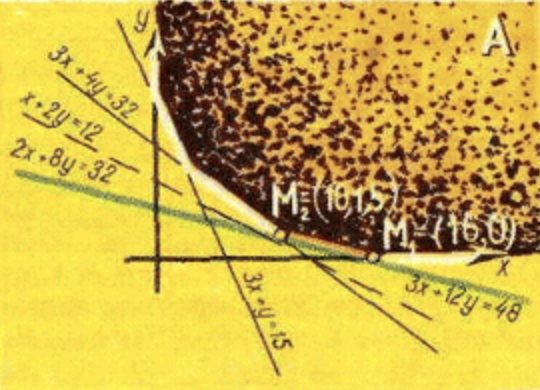
\includegraphics[width=1.0\linewidth]{image.png}
}
\newpara
 }
 \colchunk{
 Так как тангенс угла наклона прямых 3х + 12у = с совпадает с тангенсом угла наклона одной  из прямых, на которых лежат стороны множества допустимых точек (прямой 2х + 8у = 32), то опорная прямая совпадает с этой прямой. Решениями задачи служат все точки стороны, лежащей на этой прямой. Концами этой стороны служат вершины, лежащие в точках пересечения прямой 2х + 8у = 32 с соседними прямыми — у = 0 и 3х + 4у = 36 (напомним, что прямую х + 2у = 12 мы исключили из рассмотрения). Итак, координаты  (x_{1}, y_{1}) 
\vspace{0.5cm}
\breakline

\begin{equation*}
    \begin{cases}
      2x_{1} + 8y_{1} = 32 ,\\ y_{1} = 0.
      \end{cases}
\end{equation*}
}
\end{multicols}
\end{justify}

\newpara
8
